\chapter{Evaluation}

The main issue of the current implementation in Bdrive is the poor scalability of the number of file keys. For each new device, a new file key needs to be created and maintained. The proposed prototype serves as the proof-of-concept that such a distributed, secure system can exist which fits all the requirements of section \req{sec:requirements} and scales better than the current system implemented in Bdrive. 

To stress this last point, different benchmarks will be conducted to compare the proposed prototype to a similar environment such as Bdrive. The goal of this section will be to show that the assumption following assumption holds true:

\begin{center}
\textit{The ABE-based solution, of the in section \ref{sec:implementation} proposed system to solve the scalability problem of a secure cloud storage system, scales at least as good as the RSA-based approach, described in section \ref{sec:background}, regarding the number of file keys that need to be maintained.}
\end{center}

While this assumption should hold true on group operations such as member join and file upload, the proposed approach comes with an additional overhead on member removal due to additional shared-key revocation management. 

\section{Upper-Bound and Worst-Case Scenario}
\label{sec:upper-bound-and-worst-case-scenario}
In this section it will theoretically argued why \name scales at least as good as the current solution for secure cloud storage systems. The number of files keys per $n$ user scale with $O(n)$ (same way as Bdrive) in \name if and only if, no suitable subset of district attributes of any two users can be found so that the $n$ users can be described with $a < n$ attributes $a$. 
That means that if in that group at least two users would share the same attribute only $a < n$ attributes would be needed to describe this group, resulting in $a$ file keys. 
If that is not the case, say no user share the same attribute, for each user an unique attribute needs to be used (for example the email address of the user) which is embedded in an inclusive attribute policy. 

\begin{center}
\begin{lstlisting}[caption={Worst case access policy. The used email address is a unique attribute per user.},captionpos=b]
(alice@example.com OR bob@example.com OR ... OR zara@example.com)
\end{lstlisting}
\end{center}

Such policy will spawn each unique attribute of the users combining them with an "OR" (see above example). As described in section \ref{sec:extension-to-dnf-policy} this will case the creation of $n$ cipher texts, the exact same number of file keys that will also be created in Bdrive. 

The remaining assumption that needs to be shown is that for each "AND" used in the access policy the resulting number of cipher text will be effective smaller then the number of users. 

\section{Performance and Scalability Analysis}

To evaluate the performance and scalalbility of \name against the classical implementation different benchmarks are conducted. While the main focus remains on reducing the number of file keys for group sharings, it is also importend to mesure the performance of encryption, decryption, member join and member leave actions. Since encryption is the most interessing evaluation because it scales with the number of users, number of attributes, effects the cipher text length and number of file keys. In the following sections each of the four different actions will be evaluated and an expection about the experiment ourcome will be given.

The benchmark evaluation is executed on a Server machine utalizing 6 vCPU cors (Intel(R) Xeon(R) CPU E5-2680 v3 @ 2.50GHz, 30MB cache size), 12 GB RAM and running on Ubuntu 16.04 LTS 64bit. For the evaluation OpenJDK 1.8.0\_191 is used. Each of the benchmark does not spawn any threads or uses parallelisation. Computing power results from a single thread. \footnote{Single thread assumption is based on the implementation of \name. This assumption must not hold true for libraries that are used under the hood for RSA and AES cryptography (bouncycastle 1.60) or pairing-based cryptography (jPBC 2.0.0).} 

\subsection{Encryption}
Encryption is the most interessing topic to evaluate since it scales using RSA with the number of users and using ABE with the number of attriubtes. With having the assumption of section \ref{sec:comparing-secure-group-communication-to-attribute-based-encryption} in mind, that states that the number of attributes is smaller or equal to the number of users in the shared group, ABE should be albe to archive a better performance. 

\subsubsection{Assumption}
Classical encryption that uses RSA to encrypt the file key asymmetrically scales with the number of users. For each new file in the group a suitable file key for each user must be created. The resulting assumption is that the RSA based approach scales linearly with increasing number of users. Same holds true for the cipher text size. This describes the aggregated sum of all file keys for one file. The number of file keys should scale on the order of 1-to-1 with the number of users. 

In contrast to that stands \name. It scales with the number of attributes per cipher text rather then the number of users. Given this assumption an intersecting point of "attributes per user" can be calculated where \name scales better then the RSA approach. Where this intersecting point is depends on the number of attributes, number of users, the choosen policy and the computing power of the executing machine. Since in pure performance RSA computes faster then pairing-based cryptography, it can be assumped that there can be cases where there is no intersection point and the RSA-appraoch simply scales better. 

\subsubsection{Benchmark: "and"-policies}
There where two different scenarios evaluated. Frist, the and-policies (best-case) and then the or-policies (worst-case) were analysed for performance and scalability. The benchmarks are performed over an increasing number of users. For each $n$ users a new attribute is introduced. The notation of $a$-for-$n$ defining $a$ as the number of attributes \textit{for} $n$ users. The benchmark is evaluated for the configurations $1$-for-$\infty$, $1$-for-$1$, $1$-for-$2$, $1$-for-$4$, $1$-for-$5$.

% picture
\begin{figure}[!t]
\centering
    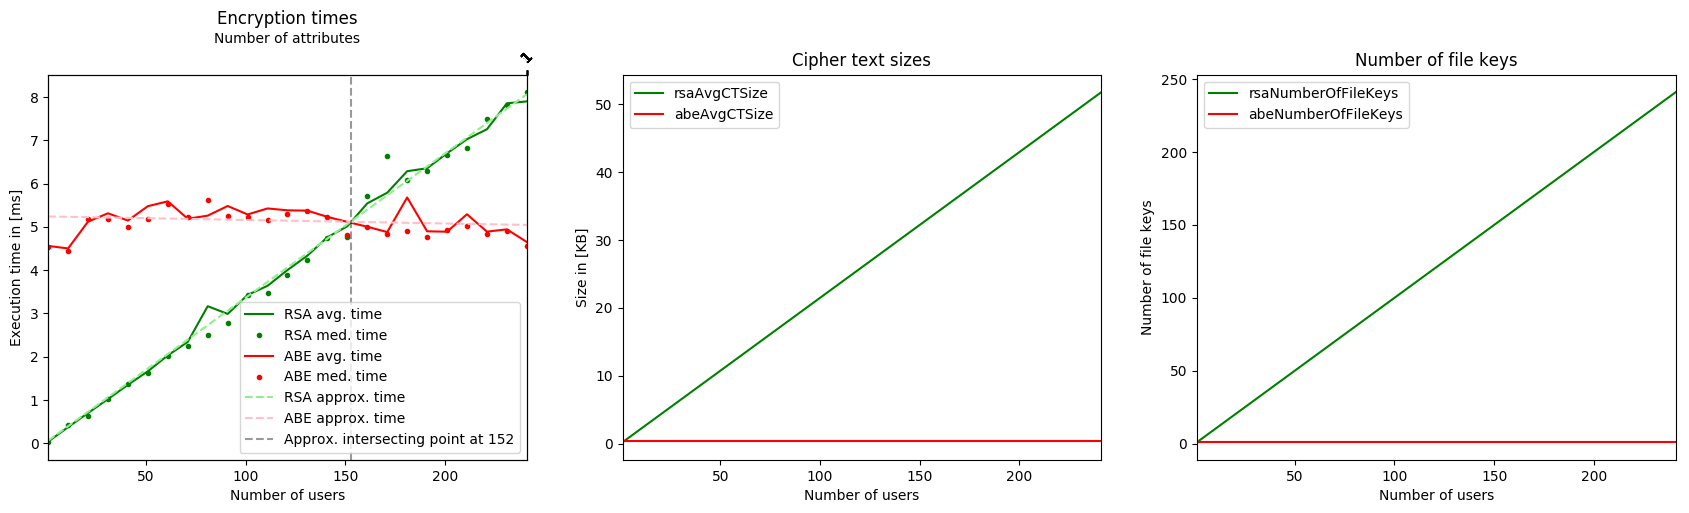
\includegraphics[width=\linewidth]{img/eval-and-policy/encrypt_incrementing_10.png}
    \caption{$1$-for-$\infty$ configuration using "and"-policy}
    \label{fig:1-for-infty-and}
\end{figure}
\begin{figure}[!t]
\centering
    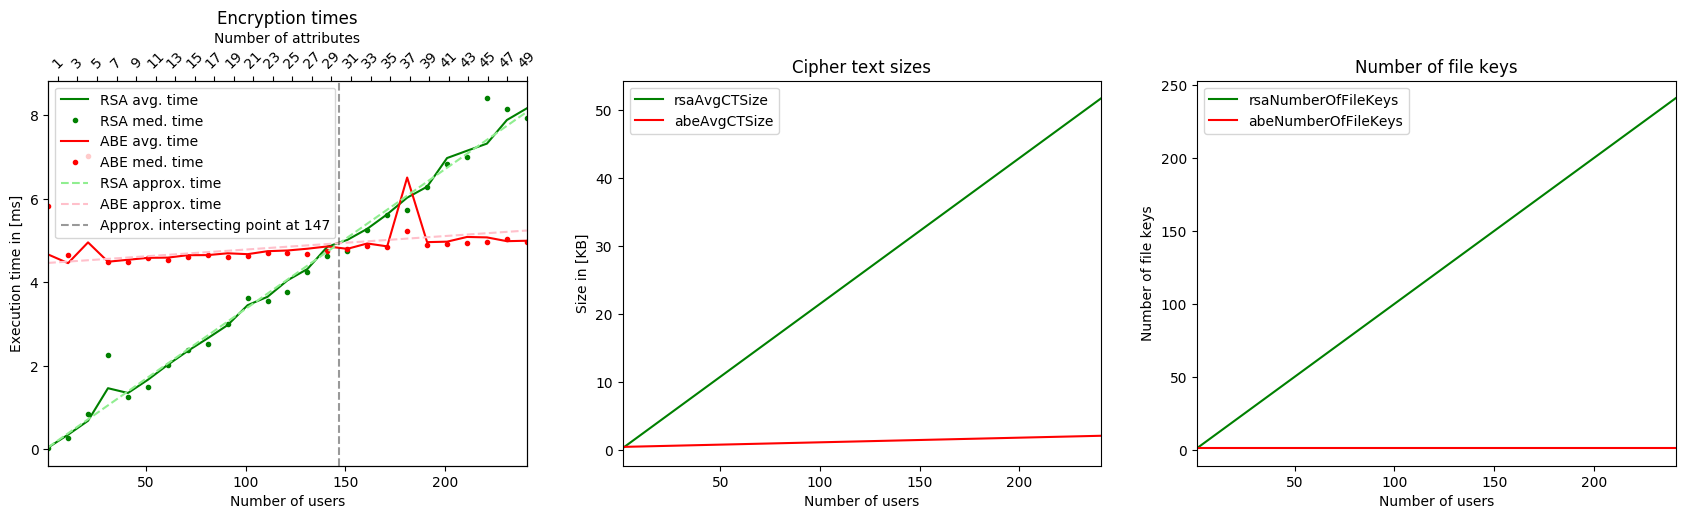
\includegraphics[width=\linewidth]{img/eval-and-policy/encrypt_incrementing_10_attribute_increment_1per5User.png}
    \caption{$1$-for-$5$ configuration using "and"-policy}
    \label{fig:1-for-5-and}
\end{figure}
\begin{figure}[!t]
\centering
    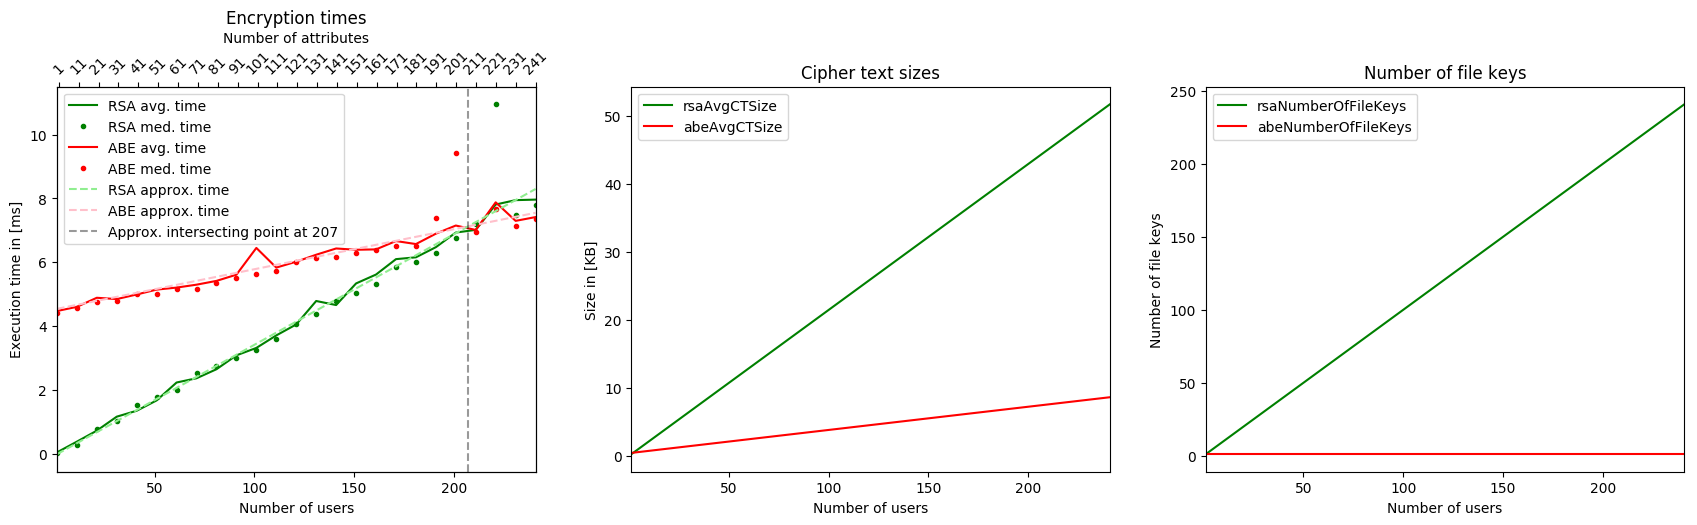
\includegraphics[width=\linewidth]{img/eval-and-policy/encrypt_incrementing_10_attribute_increment_1per1User.png}
    \caption{$1$-for-$1$ configuration using "and"-policy}
    \label{fig:1-for-1-and}
\end{figure}

The configuration of $1$-for-$\infty$ as shown in figure \ref{fig:1-for-infty-and} describes the best-case scenario. Here a group can be complelty described by only one attribute, regardless of the number of users. \name has an constant overhead since the number of attributes remain constant. The intersecting point can be approximated at 145 users. From that point onwards \name scales better then the RSA-based approach. With increasing the number of attributes per user, the overhead of \name becomes greater. In the configuration of $1$-for-$1$, so that each new user introduces a new attribute, the intersecting point gets pushed back to roughly 200 users. 

Comparing the number of file keys over the increasing number of attributes per user, it is obserable that the number of file keys indeed scale truely linearly to the number of users. \name archieves to hold the number of file keys, when using "and"-policies, constant to $1$. The cipher text size raises linearly with increasing number of attributes that need to be embedded into this policy. It still scales better then the RSA based approach. 

\subsubsection{Benchmark: "or"-policies}
\begin{figure}[!t]
\centering
    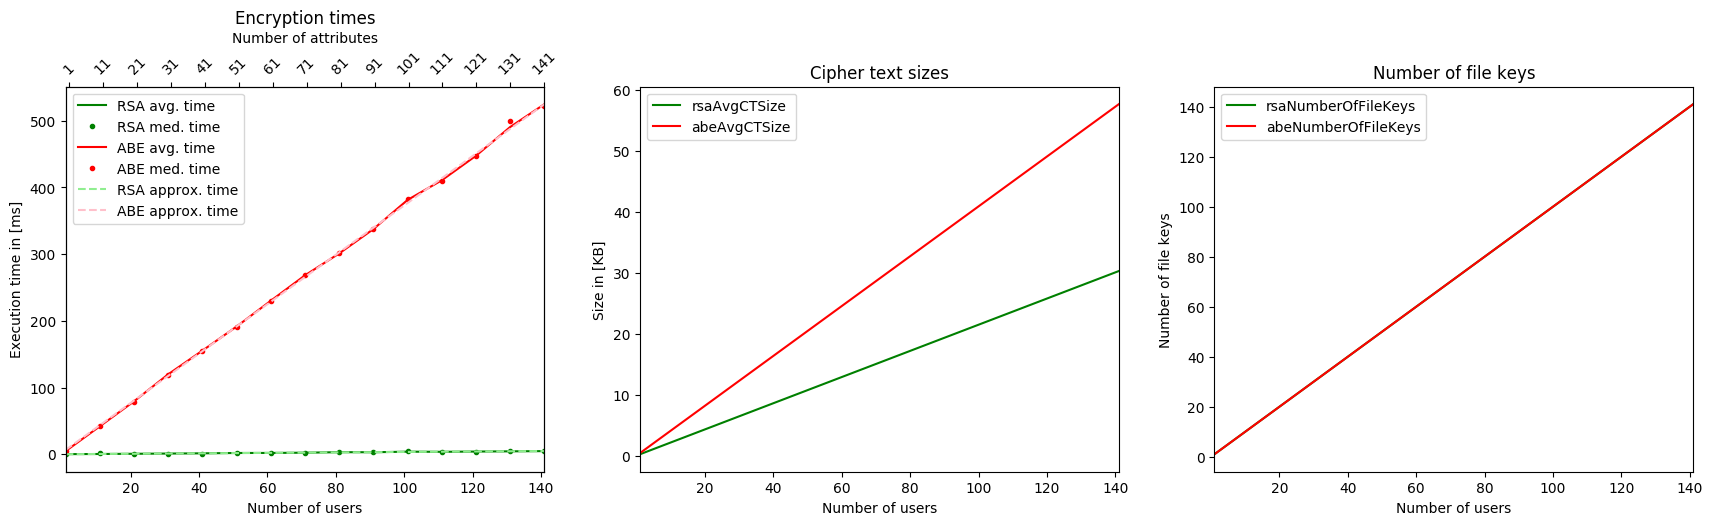
\includegraphics[width=\linewidth]{img/eval-or-policy/encrypt_incrementing_10_attribute_increment_1per1User.png}
    \caption{$1$-for-$1$ configuration using "or"-policy}
    \label{fig:1-for-1-or}
\end{figure}
\begin{figure}[!t]
\centering
    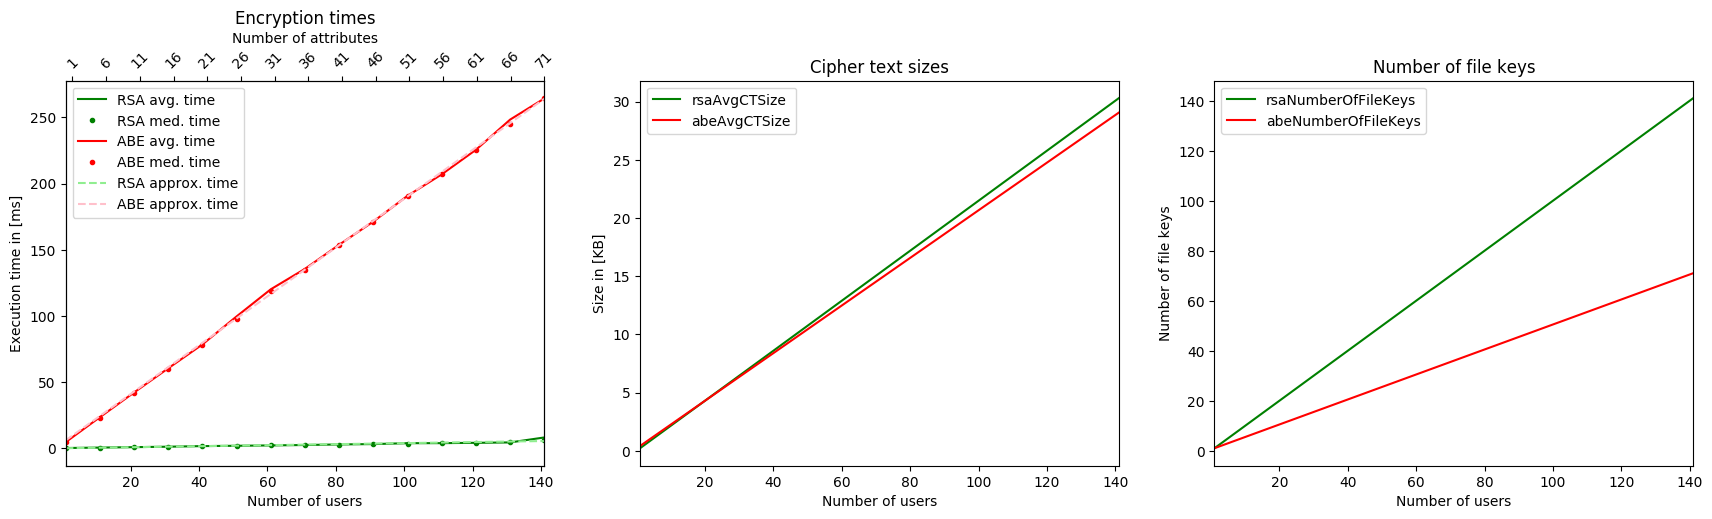
\includegraphics[width=\linewidth]{img/eval-or-policy/encrypt_incrementing_10_attribute_increment_1per2User.png}
    \caption{$1$-for-$2$ configuration using "or"-policy}
    \label{fig:1-for-2-or}
\end{figure}
\begin{figure}[!t]
\centering
    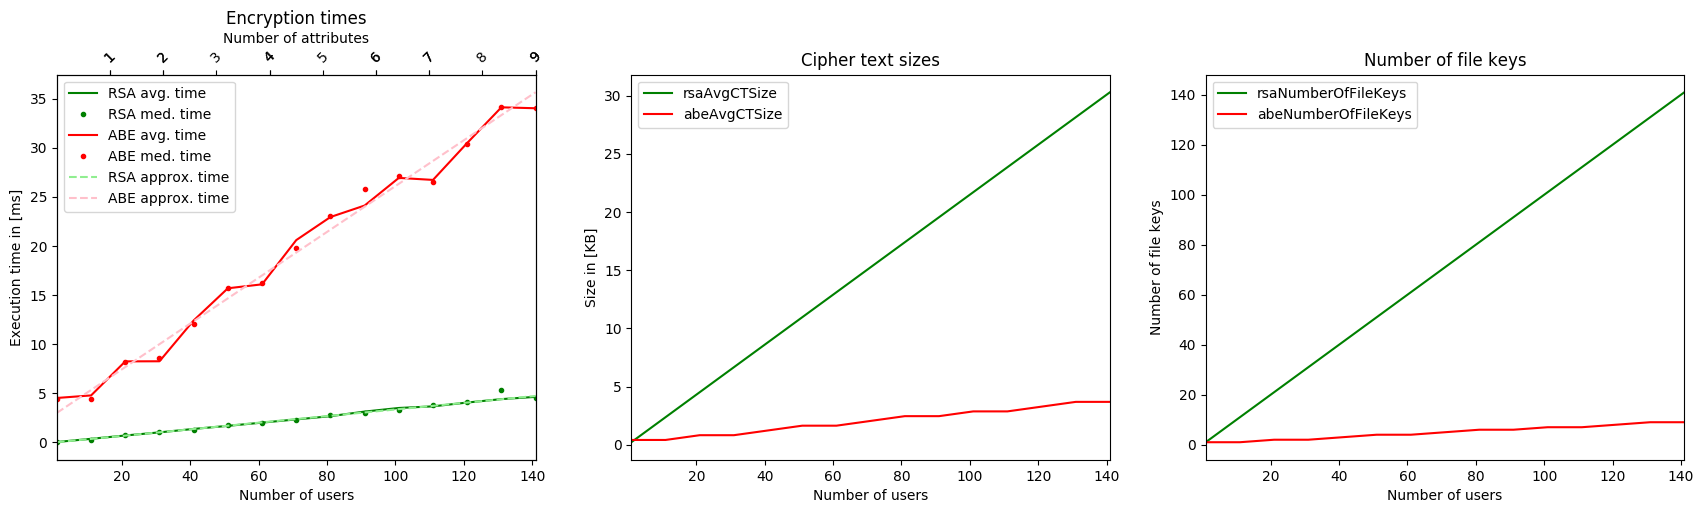
\includegraphics[width=\linewidth]{img/eval-or-policy/encrypt_incrementing_10_attribute_increment_1per16User.png}
    \caption{$1$-for-$16$ configuration using "or"-policy}
    \label{fig:1-for-16-or}
\end{figure}
\begin{figure}[!t]
\centering
    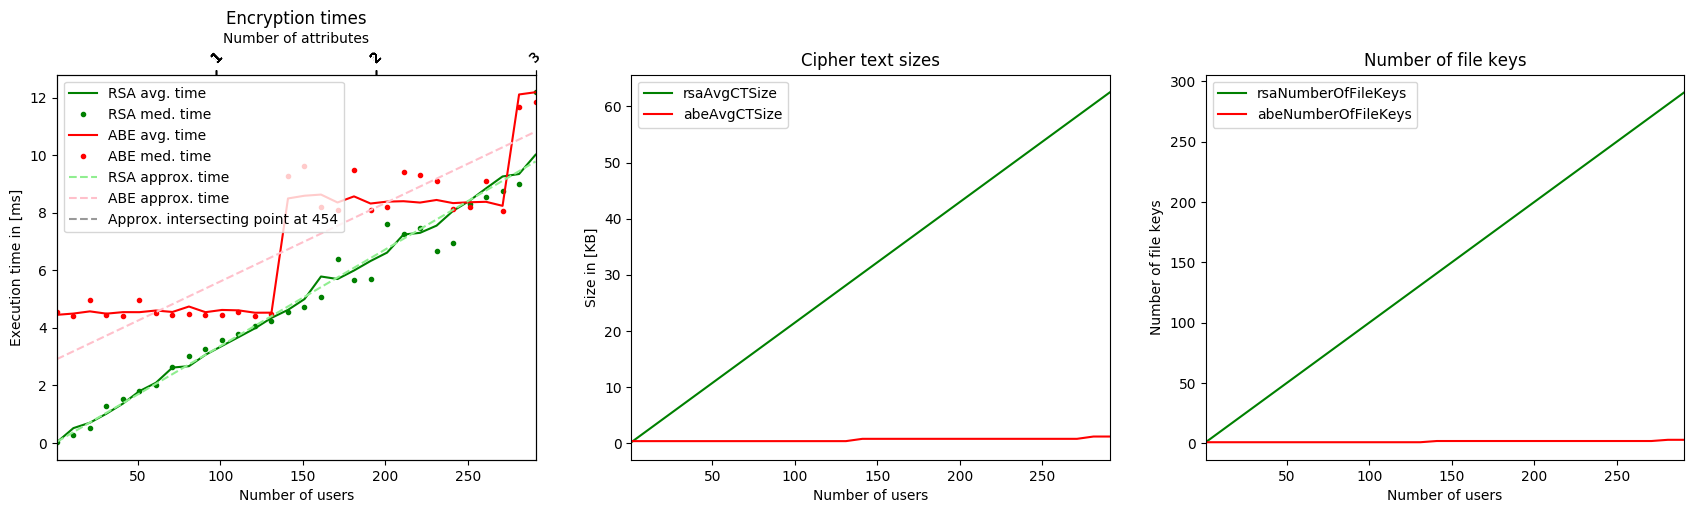
\includegraphics[width=\linewidth]{img/eval-or-policy/encrypt_incrementing_10_attribute_increment_1per140User.png}
    \caption{$1$-for-$140$ configuration using "or"-policy}
    \label{fig:1-for-140-or}
\end{figure}

Complelty different is the benchmark for "or"-policies. Since for each "or" a new cipher text needs to be created \name scales with the number of "or" elements present in the access policy.


%\begin{figure}[!t]
%\centering
%    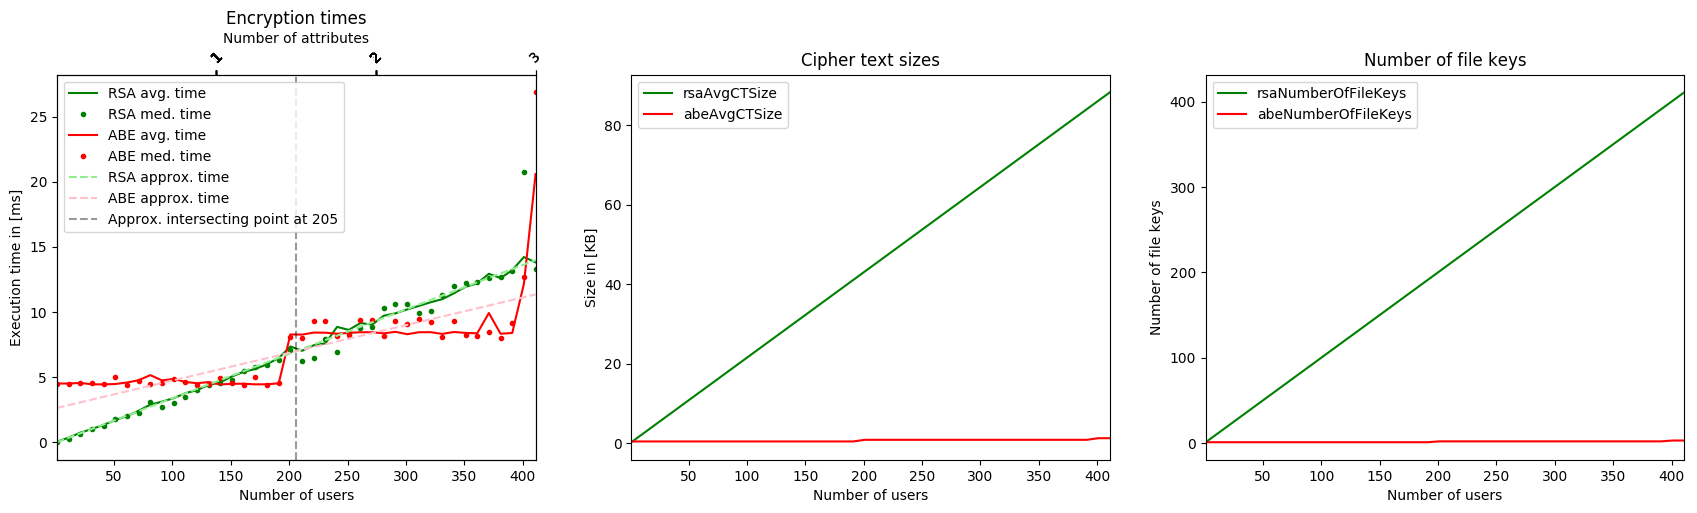
\includegraphics[width=\linewidth]{img/eval-or-policy/encrypt_incrementing_10_attribute_increment_1per200User.png}
%    \caption{$1$-for-$200$ configuration using "or"-policy}
%    \label{fig:1-for-200-or}
%\end{figure}


As it was introduced in the previous chapture, TF-DAC-MACS was adapted to support access policies that are present DNF-fomular. For each additional "or" and its suptree a new chiper text gets created. This is visible in the Figure \ref{fig:1-for-16-or} in the cipher text size and number of file key graphic. Here a stepwise increasing function is notable. Each step is directly correlated to a new attribute that was included into the policy using konjunction.

The worst-case scenario, as introduced in section \ref{sec:upper-bound-and-worst-case-scenario}, is defined as the scenarion were the number of users is equal the number of attributes in an or-policy. This case is shown in figure \ref{fig:1-for-1-or}. In that case is encryption time of \name two magintues higher ($\approx 0-550$ms) than the computation time of the RSA-approach ($\approx 0-10$ms). Even the cipher text size is substantial greater than the cipher text size per file key. This results from the fact that now, \name scales with the same overhead as the RSA approach regarding the number of file keys. So no adventage could be gained over the RSA approach in the worst-case scenario.

Interessting to notice is if a configuration of one attribute per two users is used (Figure \ref{fig:1-for-2-or}) the file keys scale twice as good and the cipher text size scale rather similar to the size of the RSA based file keys. 

Reducing the overhead to a 1-for-16 configuration using "or"-policies, as shown in Figure \ref{fig:1-for-16-or}, a step wise function is notable in each of the plottet functions. The next step happens each 16 users - each attribute. The less attributes are used to describe a user group using "or"-policies, the better does \name scale. Since the number of attributes and the number of cipher text are directly correltated, a great adventage over the classical RSA-based appraoch can be archieved.

Finally, in Figure \ref{fig:1-for-140-or}, a configuration was when \name can b expected to scale better then the RSA-based appraoch. When a group of user can be described by a policy that utalized no "or" for at least 140 members, the assumption can be made that \name scales better regarding computation time in comparison to the classical RSA-based appraoch. 

In general it holds true that the regarding the cipher text size and the number of file keys \name scales better if a group of user can be described by "or" conditions then there are users. 

\subsection{Member Join}
On member join, in RSA each file key needs to be reencrypted for the new member. Using the ABE appraoch simply a attribute key that matches the group policy needs to be created. 

\subsubsection{Assumption}
Given the previous statement, it can be assumped that \name scales with an constant overhead and the RSA approach scales linearly with the increasing number of cipher texts.

\subsubsection{Benchmark: Member Join}
\begin{figure}[!ht]
\centering
    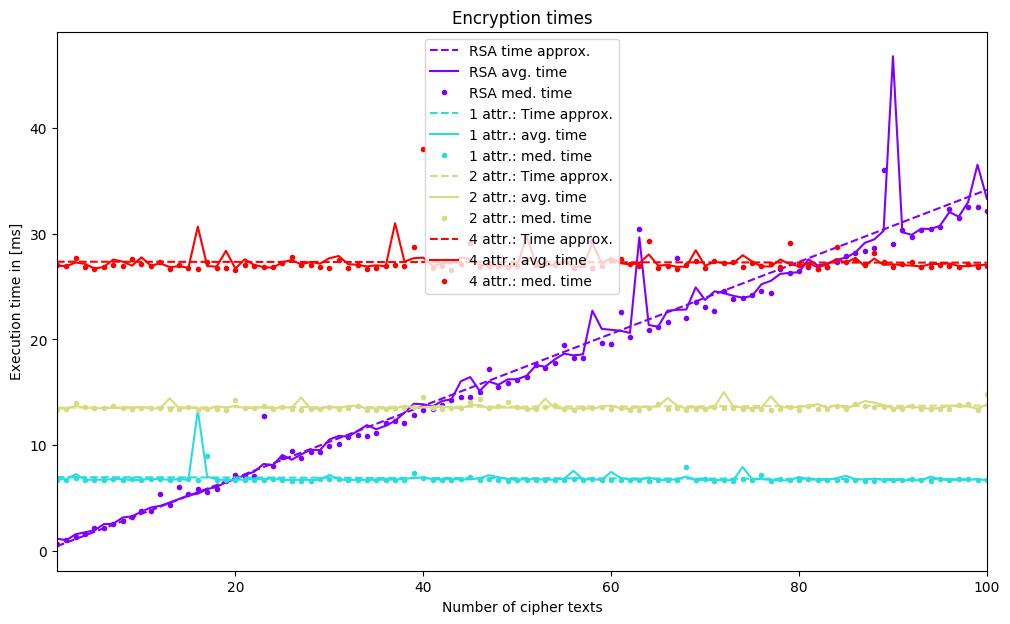
\includegraphics[width=\linewidth]{img/eval-join/join_attr_1.png}
    \caption{Rekeying for one new member. Scaled over the number of attributes}
    \label{fig:member-join}
\end{figure}

As shown in figure \ref{fig:member-join} the assumption can be supported. Three group configurations were evaluated. Having 1, 2 or 4 attributes respectivcally. Depending on the number of attributes the intersecting points of 20, 40 and 90 cipher texts can be extracted. After this amount of attributes \name is faster in adding members to a group. 

\subsection{Member Leave}
Member Leave comes with a greater overhead for \name. Additionally all cipher text need to be updated, each non-revoker user need to revieve a new update key, and the cipher text update key, user secret update key and new attribute value private and public key need to be calculated. On the other hand is the biggest adventage of the RSA-based appraoch that simply the respective file keys of the revoked user need to be deleted.

\subsubsection{Assumption}
The assumption is simply stated that \name can not scale better then the RSA-based approach. Even the attribute value key creation might take longer then just removing the saved file keys for the respektive user. 

\subsubsection{Benchmark: Member Leave}
\begin{figure}[!ht]
\centering
    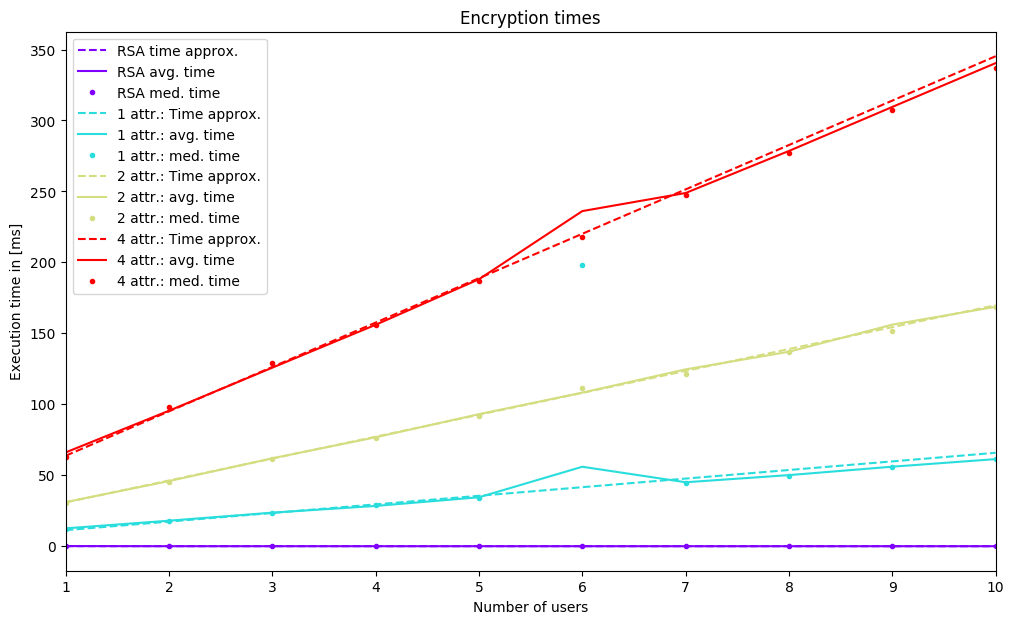
\includegraphics[width=\linewidth]{img/eval-leave/leave_attr_1_users_2.png}
    \caption{One member leaves the share. Scaled over the number of attributes}
    \label{fig:member-leave}
\end{figure}

Figure \ref{fig:member-leave} shows the exact expected behavior. For already one cipher text the gab between the different number of attributes and the RSA-based approach is crealy notable. More attributes means here that a user was revoked that owned multible attribute, which each need to be revoked by itself. 

In a real world system the cipher text update and the user secret key update would happen on the server and client device side. Further it could also happen in parallel to speed up this process. Still it holds true, that \name scales definilty much worse then the RSA-based approach.
